\documentclass[aspectratio=169,11pt]{beamer}

% Theme and colors
\usetheme{Madrid}
\usecolortheme{whale}
\setbeamertemplate{navigation symbols}{}
\setbeamertemplate{footline}[frame number]

% Packages
\usepackage[utf8]{inputenc}
\usepackage[T1]{fontenc}
\usepackage{graphicx}
\usepackage{booktabs}
\usepackage{amsmath}
\usepackage{hyperref}
\usepackage{tikz}
\usetikzlibrary{shapes,arrows,positioning,calc,fit,backgrounds}
\usepackage{siunitx}
\usepackage{xcolor}
\usepackage{array}
\usepackage{eurosym}

% Title information
\title[EECE5155 -- Module 9]{AI and MLOps for IoT}
\subtitle{Module 9: From a Trained Model to a Working IoT Product}
\author{Eduardo Baena}
\date{Spring 2026}
\institute{Northeastern University\\Department of Electrical and Computer Engineering\\
\texttt{e.baena@northeastern.edu}}

\begin{document}

% Title slide
\begin{frame}
    \titlepage
    \vspace{-1cm}
    \begin{center}
        \textbf{EECE5155: Wireless Sensor Networks and the Internet of Things}
    \end{center}
\end{frame}

%==============================================================================
\section{Learning Objectives}
%==============================================================================

\begin{frame}{Learning Objectives}
    \textbf{By the end of this module, you should be able to:}

    \vspace{0.2cm}
    \begin{enumerate}
        \item \textbf{Explain} what MLOps is and why it exists
        \item \textbf{Describe} the full lifecycle: training $\rightarrow$ deploy $\rightarrow$ monitor $\rightarrow$ retrain
        \item \textbf{Explain} why models degrade in production and how to detect it (concept drift)
        \item \textbf{Describe} how to push a new model to a deployed IoT device (OTA update)
        \item \textbf{Explain} where ML runs: cloud, gateway, or microcontroller (Edge AI)
        \item \textbf{Describe} how to improve a shared model from distributed devices (Federated Learning)
    \end{enumerate}

    \vspace{0.1cm}
    \begin{exampleblock}{Context}
        Module~8 covered how to build an ML model. This module covers \textbf{operations}: keeping a deployed model accurate on real IoT hardware over time.
    \end{exampleblock}
\end{frame}

%==============================================================================
\section{Outline}
%==============================================================================

\begin{frame}{Outline}
    \tableofcontents
\end{frame}

%==============================================================================
\section{ML in IoT: What Is a Model and How Does It Work?}
%==============================================================================

\begin{frame}{What Is a Machine Learning Model?}
    \large\textbf{Input $\rightarrow$ Model $\rightarrow$ Output}

    \vspace{0.3cm}
    \begin{center}
    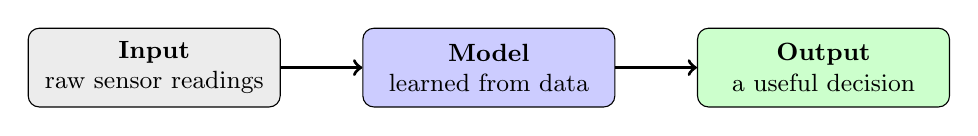
\begin{tikzpicture}[scale=0.85, every node/.style={font=\small}]
        \node[draw, fill=gray!15, minimum width=3.2cm, minimum height=1.0cm, rounded corners, align=center] (inp) at (0,0) {\textbf{Input}\\raw sensor readings};
        \node[draw, fill=blue!20, minimum width=3.2cm, minimum height=1.0cm, rounded corners, align=center] (mod) at (5.0,0) {\textbf{Model}\\learned from data};
        \node[draw, fill=green!20, minimum width=3.2cm, minimum height=1.0cm, rounded corners, align=center] (out) at (10.0,0) {\textbf{Output}\\a useful decision};
        \draw[->, very thick] (inp) -- (mod);
        \draw[->, very thick] (mod) -- (out);
    \end{tikzpicture}
    \end{center}

    \vspace{0.3cm}
    \small
    \begin{columns}
        \column{0.5\textwidth}
        \textbf{IoT examples:}
        \begin{itemize}\setlength{\itemsep}{8pt}
            \item Vibration $\rightarrow$ ``bearing fails in 5 days / OK''
            \item Temperature + occupancy $\rightarrow$ heat on / off
            \item Heart rate $\rightarrow$ ``anomaly / normal''
        \end{itemize}

        \column{0.5\textwidth}
        \begin{exampleblock}{Engineering insight}
            The model learns statistical patterns from \textbf{labeled examples}. When input data shifts beyond the training distribution, prediction quality degrades.
        \end{exampleblock}
    \end{columns}
\end{frame}

\begin{frame}{How Much Data Does a Model Need?}
    \small
    \textbf{The model learns from labeled examples. Volume is easy to collect; labels require effort.}

    \vspace{0.3cm}
    \begin{columns}
        \column{0.5\textwidth}
        \textbf{Typical amounts:}
        \begin{itemize}\setlength{\itemsep}{8pt}
            \item Simple 2-class sensor task: 500--2{,}000 examples per class
            \item Vibration fault detection: months of data + 50--200 actual fault events
            \item ``Hey Siri'' keyword: $\sim$10{,}000 voice recordings per word
        \end{itemize}

        \column{0.5\textwidth}
        \textbf{The real bottleneck: labels}
        \begin{itemize}\setlength{\itemsep}{8pt}
            \item Sensors generate data continuously; storage is cheap
            \item Every labeled example requires a human expert or a confirmed physical event
            \item At least one full year of data is needed to capture seasonal variation
        \end{itemize}

        \vspace{0.2cm}
        \begin{alertblock}{Bottom line}
            A reliable industrial model takes 6--18 months of data collection.
        \end{alertblock}
    \end{columns}
\end{frame}

\begin{frame}{Where and When Does the Model Run?}
    \small
    \textbf{Running a model on new data is called \textbf{inference}. It is very different from training.}

    \vspace{0.25cm}
    \begin{columns}
        \column{0.5\textwidth}
        \textbf{Where?}
        \begin{itemize}\setlength{\itemsep}{8pt}
            \item \textbf{Edge (on device):} real-time, no internet needed, model must be tiny
            \item \textbf{Cloud:} large model, needs network, 50--200~ms delay
        \end{itemize}

        \vspace{0.3cm}
        \textbf{When?}
        \begin{itemize}\setlength{\itemsep}{8pt}
            \item \textbf{Streaming:} every sample, every few ms; for safety and real-time alerts
            \item \textbf{Batch:} once per hour/day; for summaries, lower power consumption
        \end{itemize}

        \column{0.5\textwidth}
        \begin{exampleblock}{Two real examples}
            Safety sensor on a press machine: streaming, edge, every 10~ms.\\[6pt]
            Smart meter fraud detection: batch, cloud, once per day.
        \end{exampleblock}

        \vspace{0.3cm}
        \begin{exampleblock}{Training vs.~Inference}
            \textbf{Training:} runs periodically in the cloud; takes hours; heavy compute.\\[4pt]
            \textbf{Inference:} runs on the device; takes milliseconds; lightweight.
        \end{exampleblock}
    \end{columns}
\end{frame}

\begin{frame}{The MLOps Loop: 6 Steps}
    \small
    \textbf{The first 5 steps build the model. Step 6 keeps it working. Together they form a continuous loop.}

    \vspace{0.15cm}
    \begin{center}
    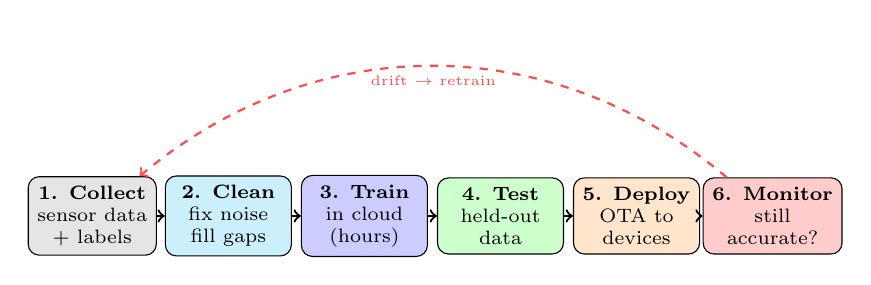
\begin{tikzpicture}[scale=0.72, every node/.style={font=\scriptsize}]
        \node[draw, fill=gray!20, minimum width=1.6cm, minimum height=0.75cm, rounded corners, align=center] (A) at (0,0)    {\textbf{1. Collect}\\sensor data\\+ labels};
        \node[draw, fill=cyan!20, minimum width=1.6cm, minimum height=0.75cm, rounded corners, align=center] (B) at (2.4,0)  {\textbf{2. Clean}\\fix noise\\fill gaps};
        \node[draw, fill=blue!20, minimum width=1.6cm, minimum height=0.75cm, rounded corners, align=center] (C) at (4.8,0)  {\textbf{3. Train}\\in cloud\\(hours)};
        \node[draw, fill=green!20, minimum width=1.6cm, minimum height=0.75cm, rounded corners, align=center] (D) at (7.2,0) {\textbf{4. Test}\\held-out\\data};
        \node[draw, fill=orange!20, minimum width=1.6cm, minimum height=0.75cm, rounded corners, align=center] (E) at (9.6,0){\textbf{5. Deploy}\\OTA to\\devices};
        \node[draw, fill=red!20, minimum width=1.6cm, minimum height=0.75cm, rounded corners, align=center] (F) at (12.0,0) {\textbf{6. Monitor}\\still\\accurate?};
        \foreach \i/\j in {A/B,B/C,C/D,D/E,E/F}
            \draw[->, thick] (\i) -- (\j);
        \draw[->, thick, dashed, red!70] (F) to[bend right=40] node[below, font=\tiny] {drift $\rightarrow$ retrain} (A);
    \end{tikzpicture}
    \end{center}

    \vspace{0.2cm}
    \begin{columns}
        \column{0.5\textwidth}
        \begin{itemize}\setlength{\itemsep}{6pt}
            \item Steps 1--5: build and deploy the model
            \item Training (step 3): cloud, offline, once per cycle
            \item Inference (step 5): on device, milliseconds, always-on
        \end{itemize}

        \column{0.5\textwidth}
        \begin{itemize}\setlength{\itemsep}{6pt}
            \item Step 6: monitor live accuracy against ground truth
            \item Accuracy drop detected $\rightarrow$ trigger step 1 again
            \item The cycle runs continuously in production
        \end{itemize}
    \end{columns}
\end{frame}

%==============================================================================
\section{What is MLOps?}
%==============================================================================

\begin{frame}{Model Degradation: The Core Engineering Problem}
    \small
    \textbf{You deploy a fault-detection model at 91\% accuracy. One year later it runs at 67\%. Same code, same hardware. What happened?}

    \vspace{0.2cm}
    \begin{columns}
        \column{0.5\textwidth}
        \textbf{Root causes:}
        \begin{itemize}\setlength{\itemsep}{4pt}
            \item Motors aged; baseline vibration signature shifted
            \item Summer temperatures changed normal operating readings
            \item Firmware update altered how the sensor encodes values
            \item Training data was collected in winter only
        \end{itemize}

        \column{0.5\textwidth}
        \begin{exampleblock}{Software vs.\ ML systems}
            A software bug triggers an exception. A degrading ML model produces plausible-looking output with reduced accuracy; the system appears healthy.
        \end{exampleblock}

        \vspace{0.2cm}
        \begin{alertblock}{Industry (2024)}
            3 out of 4 deployed IoT ML models show significant accuracy degradation within 6 months. 1 in 4 teams has automated monitoring.
        \end{alertblock}
    \end{columns}
\end{frame}

\begin{frame}{What is MLOps?}
    \small
    \textbf{MLOps = the engineering discipline of keeping a deployed ML model accurate over time.}

    \vspace{0.3cm}
    \begin{columns}
        \column{0.5\textwidth}
        \textbf{Analogy: car maintenance}
        \begin{itemize}\setlength{\itemsep}{8pt}
            \item Build the car $\equiv$ train the model
            \item Drive it $\equiv$ run inference on live data
            \item Scheduled service $\equiv$ monitor and retrain
            \item Safety recall $\equiv$ OTA model update
        \end{itemize}

        \column{0.5\textwidth}
        \begin{exampleblock}{Google Nest (2023)}
            45,000 thermostats received a faulty model update; homes were heated incorrectly. Google pushed a corrected model to all devices in 6 hours via OTA.
        \end{exampleblock}
    \end{columns}
\end{frame}

%==============================================================================
\section{The MLOps Lifecycle}
%==============================================================================

\begin{frame}[shrink]{The MLOps Lifecycle: The Continuous Loop}
    \small
    \textbf{A deployed ML system is a continuous feedback loop, not a one-time delivery.}

    \vspace{0.05cm}
    \begin{center}
    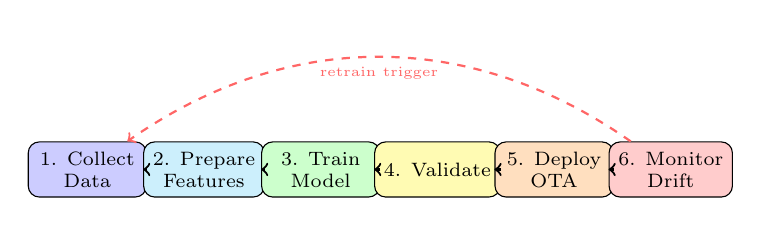
\begin{tikzpicture}[scale=0.78, every node/.style={font=\scriptsize}]
        \node[draw, fill=blue!20, minimum width=1.5cm, minimum height=0.7cm, rounded corners, align=center] (s0) at (0,0) {1. Collect\\Data};
        \node[draw, fill=cyan!20, minimum width=1.5cm, minimum height=0.7cm, rounded corners, align=center] (s1) at (1.9,0) {2. Prepare\\Features};
        \node[draw, fill=green!20, minimum width=1.5cm, minimum height=0.7cm, rounded corners, align=center] (s2) at (3.8,0) {3. Train\\Model};
        \node[draw, fill=yellow!30, minimum width=1.5cm, minimum height=0.7cm, rounded corners, align=center] (s3) at (5.7,0) {4. Validate};
        \node[draw, fill=orange!25, minimum width=1.5cm, minimum height=0.7cm, rounded corners, align=center] (s4) at (7.6,0) {5. Deploy\\OTA};
        \node[draw, fill=red!20, minimum width=1.5cm, minimum height=0.7cm, rounded corners, align=center] (s5) at (9.5,0) {6. Monitor\\Drift};
        \foreach \i in {0,1,2,3,4} {
            \pgfmathtruncatemacro{\j}{\i+1}
            \draw[->, thick] (s\i) -- (s\j);
        }
        \draw[->, thick, dashed, red!60] (s5) to[bend right=35] node[below, font=\tiny] {retrain trigger} (s0);
    \end{tikzpicture}
    \end{center}

    \begin{columns}
        \column{0.5\textwidth}
        \textbf{Each step:}
        \begin{itemize}\setlength{\itemsep}{0pt}
            \item \textbf{Collect}: sensor readings + labels (fault / OK)
            \item \textbf{Prepare}: mean, std, FFT from raw signal
            \item \textbf{Train}: fit model on historical labeled data
            \item \textbf{Validate}: test on held-out data, check accuracy
            \item \textbf{Deploy OTA}: push compiled model to device
            \item \textbf{Monitor}: compare live predictions to expected
        \end{itemize}

        \column{0.5\textwidth}
        \textbf{The loop never stops:}
        \begin{itemize}\setlength{\itemsep}{0pt}
            \item Monitoring detects drift $\rightarrow$ triggers retraining
            \item New production data $\rightarrow$ better model
            \item New model deployed $\rightarrow$ monitor again
        \end{itemize}

        \vspace{0.03cm}
        \begin{exampleblock}{Key insight}
            The model running on day~1 and the model running on day~180 are typically different versions. MLOps tracks every version deployed to every device.
        \end{exampleblock}
    \end{columns}
\end{frame}

\begin{frame}[shrink]{Why IoT Makes This Much Harder}
    \small
    \textbf{Cloud ML and IoT ML share the same algorithms but operate under completely different engineering constraints.}

    \vspace{0.2cm}
    \begin{center}
    \small
    \begin{tabular}{p{3.0cm} p{3.8cm} p{4.0cm}}
        \toprule
        \textbf{Challenge} & \textbf{Cloud ML} & \textbf{IoT ML} \\
        \midrule
        Data quality & Usually clean & Sensors drop out, gaps common \\
        Compute & Powerful GPU & Tiny chip, limited memory \\
        Network & Fast, always-on & Slow, intermittent \\
        Updates & Automatic & Must reach every device remotely \\
        Privacy & Data on your server & Health data must stay on device \\
        Scale & One server & 100,000+ different devices \\
        \bottomrule
    \end{tabular}
    \end{center}

    \vspace{0.15cm}
    \begin{exampleblock}{Engineering takeaway}
        Standard ML toolchains target cloud infrastructure. IoT deployments require rethinking compute, bandwidth, update pipelines, and data governance.
    \end{exampleblock}
\end{frame}

%==============================================================================
\section{Concept Drift}
%==============================================================================

\begin{frame}{Concept Drift: When the World Moves and the Model Does Not}
    \small
    \textbf{Model weights are fixed at training time. The physical world evolves continuously.}

    \vspace{0.25cm}
    \begin{columns}
        \column{0.5\textwidth}
        \textbf{Common causes in IoT:}
        \begin{itemize}\setlength{\itemsep}{8pt}
            \item Seasonal shift: summer vibration spectrum differs from winter
            \item Sensor aging: ADC gain drifts over months
            \item Process change: machine now operates at 60\% rated speed
        \end{itemize}

        \column{0.5\textwidth}
        \textbf{Detection signals:}
        \begin{itemize}\setlength{\itemsep}{8pt}
            \item Prediction accuracy declines gradually over weeks
            \item Output distribution shifts (e.g.\ over-predicts ``normal'')
            \item Confirmed fault events are missed by the model
        \end{itemize}

        \vspace{0.2cm}
        \textbf{Response:}
        \begin{itemize}\setlength{\itemsep}{8pt}
            \item Collect fresh labeled data under current conditions
            \item Retrain $\rightarrow$ validate $\rightarrow$ deploy via OTA
        \end{itemize}
    \end{columns}
\end{frame}

\begin{frame}[shrink]{Concept Drift: A Visual Intuition}
    \small
    \textbf{The model learned the decision boundary in January. By July, the underlying data distribution has shifted.}

    \vspace{0.05cm}
    \begin{center}
    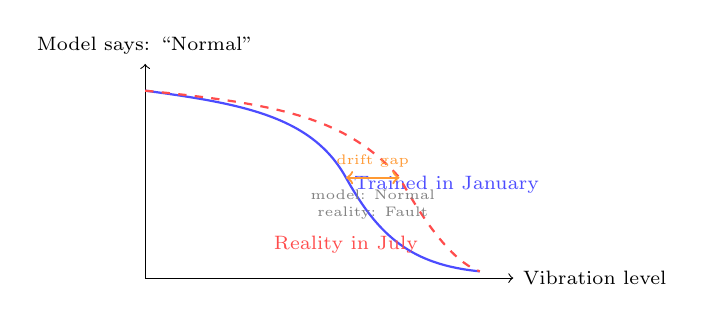
\begin{tikzpicture}[scale=0.85, every node/.style={font=\scriptsize}]
        \draw[->] (0,0) -- (5.5,0) node[right] {Vibration level};
        \draw[->] (0,0) -- (0,3.2) node[above] {Model says: ``Normal''};

        \draw[blue!70, thick] (0,2.8) .. controls (1.5,2.6) and (2.5,2.4) .. (3.0,1.5)
            .. controls (3.5,0.6) and (4.0,0.2) .. (5.0,0.1);
        \node[blue!70] at (4.5,1.4) {Trained in January};

        \draw[red!70, thick, dashed] (0,2.8) .. controls (2.0,2.6) and (3.0,2.4) .. (3.8,1.5)
            .. controls (4.3,0.6) and (4.7,0.2) .. (5.0,0.1);
        \node[red!70] at (3.0,0.5) {Reality in July};

        \draw[<->, orange!80, thick] (3.0,1.5) -- (3.8,1.5) node[midway, above, font=\tiny] {drift gap};
        \node[font=\tiny, gray, align=center] at (3.4,1.1) {model: Normal\\reality: Fault};
    \end{tikzpicture}
    \end{center}

    \vspace{0.05cm}
    \begin{columns}
        \column{0.5\textwidth}
        In January, that vibration amplitude indicated a fault condition.\\
        By July, thermal expansion shifts the baseline. The same amplitude is now within normal operating range.\\[4pt]
        \textbf{Result: false alarm rate increases 4$\times$ until the model is retrained.}

        \column{0.5\textwidth}
        \begin{alertblock}{Industry data (2024)}
            3 out of 4 deployed industrial IoT models showed drift within 6 months. Teams retraining on a 45-day cadence with fresh labeled data maintain stable accuracy.
        \end{alertblock}
    \end{columns}
\end{frame}

%==============================================================================
\section{OTA Model Updates}
%==============================================================================

\begin{frame}[shrink]{OTA Updates: Sending a New Model to Every Device Remotely}
    \small
    \textbf{OTA = Over-The-Air update. The same mechanism as a phone OS update, applied to the ML model running on an embedded sensor.}

    \vspace{0.05cm}
    \begin{center}
    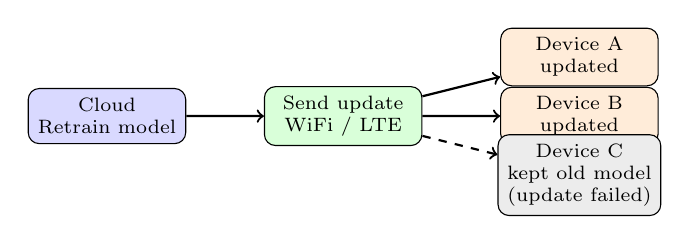
\begin{tikzpicture}[scale=0.75, every node/.style={font=\scriptsize}]
        \node[draw, fill=blue!15, minimum width=2cm, minimum height=0.7cm, rounded corners, align=center] (cloud) at (0,1.5) {Cloud\\Retrain model};
        \node[draw, fill=green!15, minimum width=2cm, minimum height=0.7cm, rounded corners, align=center] (broker) at (4,1.5) {Send update\\WiFi / LTE};
        \node[draw, fill=orange!15, minimum width=2cm, minimum height=0.7cm, rounded corners, align=center] (dev1) at (8,2.5) {Device A\\updated};
        \node[draw, fill=orange!15, minimum width=2cm, minimum height=0.7cm, rounded corners, align=center] (dev2) at (8,1.5) {Device B\\updated};
        \node[draw, fill=gray!15, minimum width=2cm, minimum height=0.7cm, rounded corners, align=center] (dev3) at (8,0.5) {Device C\\kept old model\\(update failed)};
        \draw[->, thick] (cloud) -- (broker);
        \draw[->, thick] (broker) -- (dev1);
        \draw[->, thick] (broker) -- (dev2);
        \draw[->, thick, dashed] (broker) -- (dev3);
    \end{tikzpicture}
    \end{center}

    \vspace{0.05cm}
    \begin{columns}
        \column{0.5\textwidth}
        \textbf{How it works:}
        \begin{enumerate}\setlength{\itemsep}{2pt}
            \item Drift detected $\rightarrow$ trigger retrain in cloud
            \item Package and sign model binary for target hardware
            \item Transmit wirelessly; device checks integrity before install
            \item On failure: device retains previous model version
        \end{enumerate}

        \column{0.5\textwidth}
        \textbf{Always roll out gradually:}
        \begin{itemize}\setlength{\itemsep}{2pt}
            \item Deploy to 1\% of fleet; monitor for 24 hours
            \item Expand to 10\%, then 100\% if metrics hold
            \item Automated rollback if error rate rises
        \end{itemize}
        \vspace{0.08cm}
        \begin{exampleblock}{Tesla Autopilot}
            Every neural network update reaches 1.5M+ vehicles via staged rollout with per-vehicle telemetry monitoring.
        \end{exampleblock}
    \end{columns}
\end{frame}

%==============================================================================
\section{Where Does ML Run? Edge AI}
%==============================================================================

\begin{frame}[shrink]{Where Does the Model Run?}
    \small
    \textbf{Inference can run at any tier from the sensor itself to the cloud. The right tier depends on latency, power, bandwidth, and privacy requirements.}

    \vspace{0.02cm}
    \begin{center}
    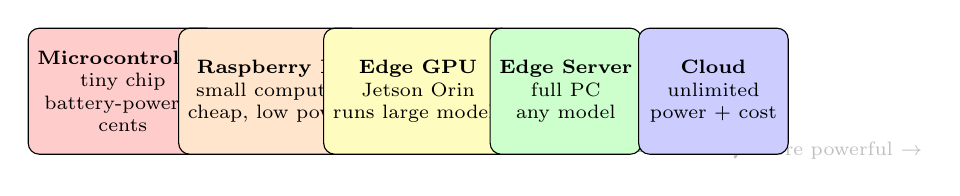
\begin{tikzpicture}[scale=0.75, every node/.style={font=\scriptsize}]
        \draw[->, very thick, gray!50] (-0.3,0) -- (11.5,0) node[right] {More powerful $\rightarrow$};

        \node[draw, fill=red!20, minimum width=1.9cm, minimum height=1.6cm, rounded corners, align=center] at (1,1.0) {\textbf{Microcontroller}\\tiny chip\\battery-powered\\cents};
        \node[draw, fill=orange!20, minimum width=1.9cm, minimum height=1.6cm, rounded corners, align=center] at (3.5,1.0) {\textbf{Raspberry Pi}\\small computer\\cheap, low power};
        \node[draw, fill=yellow!25, minimum width=1.9cm, minimum height=1.6cm, rounded corners, align=center] at (6.0,1.0) {\textbf{Edge GPU}\\Jetson Orin\\runs large models};
        \node[draw, fill=green!20, minimum width=1.9cm, minimum height=1.6cm, rounded corners, align=center] at (8.5,1.0) {\textbf{Edge Server}\\full PC\\any model};
        \node[draw, fill=blue!20, minimum width=1.9cm, minimum height=1.6cm, rounded corners, align=center] at (11.0,1.0) {\textbf{Cloud}\\unlimited\\power + cost};
    \end{tikzpicture}
    \end{center}

    \vspace{0.05cm}
    \begin{columns}
        \column{0.5\textwidth}
        \textbf{Advantages of edge inference:}
        \begin{itemize}\setlength{\itemsep}{0pt}
            \item \textbf{Latency}: sub-millisecond response, no round-trip
            \item \textbf{Bandwidth}: transmit one score, retain raw data locally
            \item \textbf{Privacy}: sensor data stays on device
            \item \textbf{Resilience}: operates without network connectivity
        \end{itemize}

        \column{0.5\textwidth}
        \textbf{Engineering tradeoff:}
        \begin{itemize}\setlength{\itemsep}{0pt}
            \item Constrained hardware limits model complexity
            \item Microcontroller: simple classifiers, TinyML
            \item Raspberry Pi class: medium CNNs, LSTM
            \item Cloud: unlimited complexity, adds latency
        \end{itemize}
        \vspace{0.05cm}
        \begin{exampleblock}{Design rule}
            Deploy inference as close to the sensor as accuracy and power budget allow.
        \end{exampleblock}
    \end{columns}
\end{frame}

\begin{frame}[shrink]{TinyML: Running AI on a Tiny Chip}
    \small
    \textbf{Standard model: $\sim$100 MB. Sensor MCU flash: $\sim$256 kB. TinyML closes the gap via two key techniques.}

    \vspace{0.2cm}
    \begin{columns}
        \column{0.5\textwidth}
        \textbf{Quantization (precision reduction):}
        \begin{itemize}\setlength{\itemsep}{8pt}
            \item Weights: FP32 $\rightarrow$ INT8 (4$\times$ smaller)
            \item Accuracy loss: $<$1\% on most IoT tasks
            \item Analogy: RAW $\rightarrow$ JPEG; same image, lower bitrate
        \end{itemize}

        \vspace{0.2cm}
        \textbf{Pruning (weight sparsification):}
        \begin{itemize}\setlength{\itemsep}{8pt}
            \item 80--90\% of weights are near zero; set to zero and skip
            \item Structured pruning reduces compute; unstructured reduces size
        \end{itemize}

        \column{0.5\textwidth}
        \textbf{Deployed today on MCUs:}
        \begin{itemize}\setlength{\itemsep}{8pt}
            \item Gesture recognition on Arduino Nano 33 BLE
            \item Keyword detection on a chip smaller than a fingernail
            \item Vibration anomaly on a \$3 MEMS sensor module
        \end{itemize}

        \vspace{0.15cm}
        \begin{exampleblock}{Toolchains}
            \textbf{Edge Impulse}: end-to-end: collect, train, quantize, deploy.\\[4pt]
            \textbf{TFLite Micro}: Google runtime for microcontrollers.
        \end{exampleblock}
    \end{columns}
\end{frame}

%==============================================================================
\section{Federated Learning}
%==============================================================================

\begin{frame}[shrink]{Federated Learning: Training Without Sharing Private Data}
    \small
    \textbf{When raw data is privacy-sensitive or too large to transmit, training must happen on-device.}

    \vspace{0.1cm}
    \begin{columns}
        \column{0.5\textwidth}
        \textbf{Centralized training:}
        \begin{itemize}\setlength{\itemsep}{6pt}
            \item Aggregate raw data from all devices to a central server
            \item Train on the full dataset
            \item Constrained by: HIPAA, CCPA, industrial trade secrets
        \end{itemize}

        \vspace{0.15cm}
        \textbf{Federated Learning:}
        \begin{itemize}\setlength{\itemsep}{6pt}
            \item Raw data remains on each device
            \item Local training produces \textbf{model weight updates}
            \item Server aggregates updates $\rightarrow$ improved global model $\rightarrow$ redistribute. Repeat.
        \end{itemize}

        \column{0.5\textwidth}
        \begin{center}
        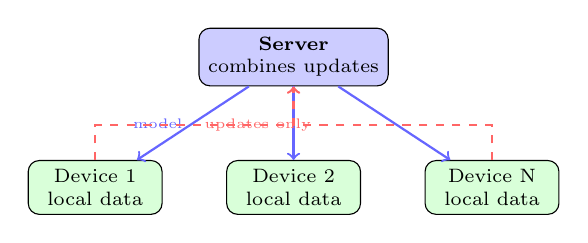
\begin{tikzpicture}[scale=0.72, every node/.style={font=\scriptsize}]
            \node[draw, fill=blue!20, minimum width=2.0cm, minimum height=0.65cm, rounded corners, align=center] (server) at (4.5,2.8) {\textbf{Server}\\combines updates};
            \node[draw, fill=green!15, minimum width=1.7cm, minimum height=0.6cm, rounded corners, align=center] (d1) at (1,0.5) {Device 1\\local data};
            \node[draw, fill=green!15, minimum width=1.7cm, minimum height=0.6cm, rounded corners, align=center] (d2) at (4.5,0.5) {Device 2\\local data};
            \node[draw, fill=green!15, minimum width=1.7cm, minimum height=0.6cm, rounded corners, align=center] (d3) at (8.0,0.5) {Device N\\local data};
            \draw[->, blue!60, thick] (server) -- (d1) node[midway, left, font=\tiny] {model};
            \draw[->, blue!60, thick] (server) -- (d2);
            \draw[->, blue!60, thick] (server) -- (d3);
            \draw[->, red!60, thick, dashed] (d1) -- ++(0,1.1) -| (server) node[near start, right, font=\tiny] {updates only};
            \draw[->, red!60, thick, dashed] (d3) -- ++(0,1.1) -| (server);
        \end{tikzpicture}
        \end{center}

        \begin{exampleblock}{Google Keyboard (Gboard)}
            500 million Android devices. Keystroke data stays on-device. Only gradient updates are aggregated. Model quality matches centralized training within 2\%.
        \end{exampleblock}
    \end{columns}
\end{frame}

\begin{frame}{Federated Learning: Why It Matters for IoT}
    \small
    \textbf{Federated Learning simultaneously addresses three IoT constraints.}

    \vspace{0.25cm}
    \begin{columns}
        \column{0.5\textwidth}
        \textbf{Privacy:} raw data stays on device; compliant by architecture\\[6pt]
        \textbf{Bandwidth:} weight updates are 1{,}000$\times$ smaller than raw sensor streams\\[6pt]
        \textbf{Compliance:} HIPAA, CCPA satisfied without legal review of each transfer

        \vspace{0.2cm}
        \textbf{Accuracy trade-off:} 2--5\% below centralized baseline; acceptable for most IoT tasks

        \column{0.5\textwidth}
        \begin{exampleblock}{Production deployments (2025)}
            Google (Gboard), Apple (Siri voice models), NVIDIA FLARE (hospital imaging), Amazon Halo (fitness wearable).
        \end{exampleblock}
    \end{columns}
\end{frame}
\section{End-to-End Case Studies}
%==============================================================================

\begin{frame}{Case Study 1: Predicting Machine Failures Before They Happen}
    \small
    \textbf{500 CNC machines, each with a vibration sensor. Engineering goal: predict bearing failure 5+ days ahead to enable scheduled maintenance.}

    \vspace{0.05cm}
    \begin{center}
    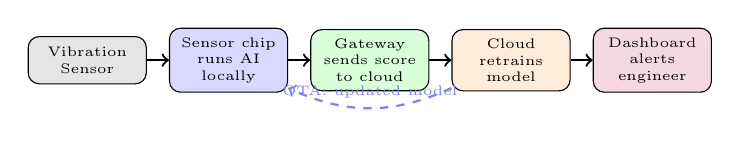
\begin{tikzpicture}[scale=0.78, every node/.style={font=\tiny}]
        \node[draw, fill=gray!20, minimum width=1.5cm, minimum height=0.6cm, rounded corners, align=center] (sensor) at (0,0) {Vibration\\Sensor};
        \node[draw, fill=blue!15, minimum width=1.5cm, minimum height=0.6cm, rounded corners, align=center] (edge) at (2.3,0) {Sensor chip\\runs AI\\locally};
        \node[draw, fill=green!15, minimum width=1.5cm, minimum height=0.6cm, rounded corners, align=center] (gw) at (4.6,0) {Gateway\\sends score\\to cloud};
        \node[draw, fill=orange!15, minimum width=1.5cm, minimum height=0.6cm, rounded corners, align=center] (ml) at (6.9,0) {Cloud\\retrains\\model};
        \node[draw, fill=purple!15, minimum width=1.5cm, minimum height=0.6cm, rounded corners, align=center] (dash) at (9.2,0) {Dashboard\\alerts\\engineer};
        \draw[->, thick] (sensor) -- (edge);
        \draw[->, thick] (edge) -- (gw);
        \draw[->, thick] (gw) -- (ml);
        \draw[->, thick] (ml) -- (dash);
        \draw[->, thick, dashed, blue!50] (ml) to[bend left=25] node[above, font=\tiny] {OTA: updated model} (edge);
    \end{tikzpicture}
    \end{center}

    \vspace{0.05cm}
    \begin{columns}
        \column{0.5\textwidth}
        \textbf{How it works:}
        \begin{itemize}\setlength{\itemsep}{0pt}
            \item Edge chip runs inference locally; transmits only a fault-probability score
            \item Cloud pipeline monitors score distribution; triggers retrain on drift
            \item Updated model pushed to all 500 devices via OTA in one cycle
        \end{itemize}

        \column{0.5\textwidth}
        \textbf{Results:}
        \begin{itemize}\setlength{\itemsep}{0pt}
            \item Failures predicted \textbf{5--8 days} before they happen
            \item Unplanned breakdowns reduced by \textbf{62\%}
            \item Maintenance costs cut by \textbf{40\%}
            \item Full model update reaches all 500 machines in 4 hours
        \end{itemize}
    \end{columns}
\end{frame}

\begin{frame}[shrink]{Case Study 2: Detecting Energy Theft Without Seeing Anyone's Data}
    \small
    \textbf{50,000 smart meters. Engineering goal: detect energy theft while keeping per-household consumption data private under CCPA.}

    \vspace{0.1cm}
    \begin{columns}
        \column{0.5\textwidth}
        \textbf{The problem:}
        \begin{itemize}\setlength{\itemsep}{0pt}
            \item Consumption profiles reveal occupancy, behaviour patterns
            \item CCPA classifies energy-usage data as personal information
            \item NB-IoT link budget limits raw data transmission
            \item 50,000 heterogeneous consumption patterns
        \end{itemize}

        \vspace{0.1cm}
        \textbf{Architecture: Federated Learning}
        \begin{itemize}\setlength{\itemsep}{0pt}
            \item Each meter trains a local anomaly model on 30 days of its own data
            \item Only model weight updates are transmitted
            \item Server aggregates updates from all 50,000 meters
        \end{itemize}

        \column{0.5\textwidth}
        \textbf{Results:}
        \begin{itemize}\setlength{\itemsep}{0pt}
            \item Theft detection accuracy: \textbf{88\%}
            \item Centralized oracle (with all data): 94\%; gap = 6\%
            \item Zero raw consumption records stored server-side
        \end{itemize}

        \vspace{0.1cm}
        \begin{exampleblock}{Engineering outcome}
            Federated architecture achieves utility-grade detection accuracy while satisfying CCPA data minimisation requirements by design.
        \end{exampleblock}
    \end{columns}
\end{frame}

%==============================================================================
\section{Responsible AI in IoT}
%==============================================================================

\begin{frame}[shrink]{Responsible AI: Your Model Affects Real People}
    \small
    \textbf{A model deployed on thousands of devices has system-level consequences when accuracy degrades.}

    \vspace{0.2cm}
    \begin{columns}
        \column{0.5\textwidth}
        \textbf{Training data bias:}
        \begin{itemize}\setlength{\itemsep}{8pt}
            \item FDA study: pulse oximeter 3$\times$ less accurate on darker skin due to underrepresentation in training cohort
            \item Training set must cover the full operational population
        \end{itemize}

        \vspace{0.2cm}
        \textbf{Auditability:}
        \begin{itemize}\setlength{\itemsep}{8pt}
            \item Model prediction alone is insufficient for liability purposes
            \item Required: model version, training dataset, deployment timestamp
        \end{itemize}

        \column{0.5\textwidth}
        \textbf{Minimum model card:}
        \begin{itemize}\setlength{\itemsep}{8pt}
            \item Model version per device (serial level)
            \item Training dataset description and date range
            \item Known failure modes and out-of-distribution conditions
            \item Accuracy log across deployment lifetime
        \end{itemize}

        \vspace{0.1cm}
        \begin{alertblock}{US regulatory context}
            FDA 510(k) requires model cards for AI medical devices. FTC Act covers consumer AI. Product liability applies to documented AI failures.
        \end{alertblock}
    \end{columns}
\end{frame}

%==============================================================================
\section{Summary}
%==============================================================================

\begin{frame}{Module 9 Summary}
    \small
    \begin{columns}
        \column{0.5\textwidth}
        \begin{itemize}\setlength{\itemsep}{10pt}
            \item \textbf{Model degradation:} 3 in 4 IoT models drift within 6 months; requires active monitoring
            \item \textbf{MLOps loop:} monitor $\rightarrow$ detect drift $\rightarrow$ retrain $\rightarrow$ OTA deploy
            \item \textbf{OTA:} staged rollout to 1\% fleet first; automated rollback on regression
        \end{itemize}

        \column{0.5\textwidth}
        \begin{itemize}\setlength{\itemsep}{10pt}
            \item \textbf{Edge AI / TinyML:} inference on MCU via quantization (FP32$\rightarrow$INT8) and pruning
            \item \textbf{Federated Learning:} aggregate weight updates; raw data stays on device
            \item \textbf{Model documentation:} version, training data, failure modes, accuracy log
        \end{itemize}
    \end{columns}

    \vspace{0.3cm}
    \begin{exampleblock}{The engineering arc}
        Module~8: build and validate a model. Module~9: operate it reliably at scale over time.
    \end{exampleblock}
\end{frame}

\begin{frame}{Questions?}
    \begin{center}
        \Huge Questions?

        \vspace{0.8cm}
        \normalsize
        \textbf{Eduardo Baena}\\
        \texttt{e.baena@northeastern.edu}\\[0.3cm]
        \textit{This concludes the IoT Data Pipeline modules (6--9).}\\
        \textit{Next: Final project presentations.}
    \end{center}
\end{frame}

\end{document}
